%!TEX root = ../thesis.tex

% \vspace{-1pt}

\section{本章の概要}
本章では,移動ロボットのナビゲーションで予測結果を利用する実験を行い,その結果を評価する.まず,実験の概要と方法について説明し,次に実験シナリオと使用したシミュレータ環境について述べる.最後に,実験結果を踏まえて考察を行う.

\section{実験概要}
予測結果を応用したナビゲーションシステムによって,移動ロボットの挙動がどのように変化するかを観察・評価するための実験を行う.実験では,2つのナビゲーションシナリオで移動ロボットを自律走行させ,各シナリオにつき10回ずつ走行を実施してデータを取得した.

\section{実験方法}
本実験の予測には,\ref{chap:proposed_method}章で提案したネットワークを用いた.ただし,使用したモデルはホールドアウト(Hold Out)方式で学習を行った.それ以外は同様の学習条件である.
また,\ref{chap:application}章で述べたシステムを用いて,ナビゲーションに予測結果を適用した.

実験は\figref{Fig:sim-env}に示すように,Gazebo\cite{Gazebo62:online}のシミュレータ環境上で行う.また,\figref{Fig:sim-robot}に示すように,シミュレータで再現した移動ロボット(ORNE-box2\cite{井口颯人2023屋外自律移動ロボットプラットフォーム-orne})を用い,歩行者は\figref{Fig:sim-actor}に示すGazeboのプラグイン\cite{Actors-G87:online}を使用してシミュレータ内に配置した.

\begin{figure}[H]
  \centering
 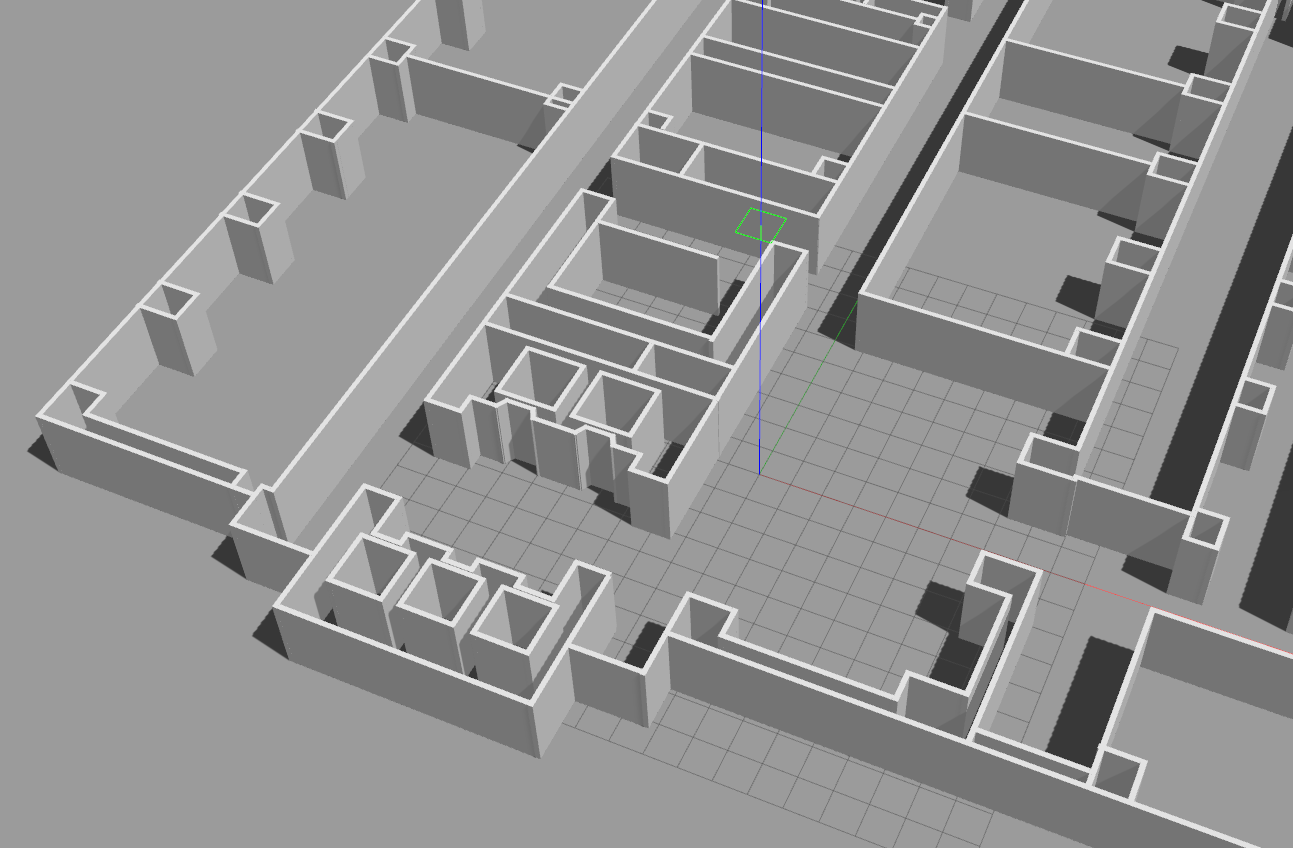
\includegraphics[keepaspectratio, scale=0.15]
      {images/sim-env.png}
\caption{Simulator environment}
 \label{Fig:sim-env}
\end{figure} 

\vspace{-10pt}

\begin{figure}[H]
  \centering
  \begin{subfigure}{0.40\textwidth}
    \centering
    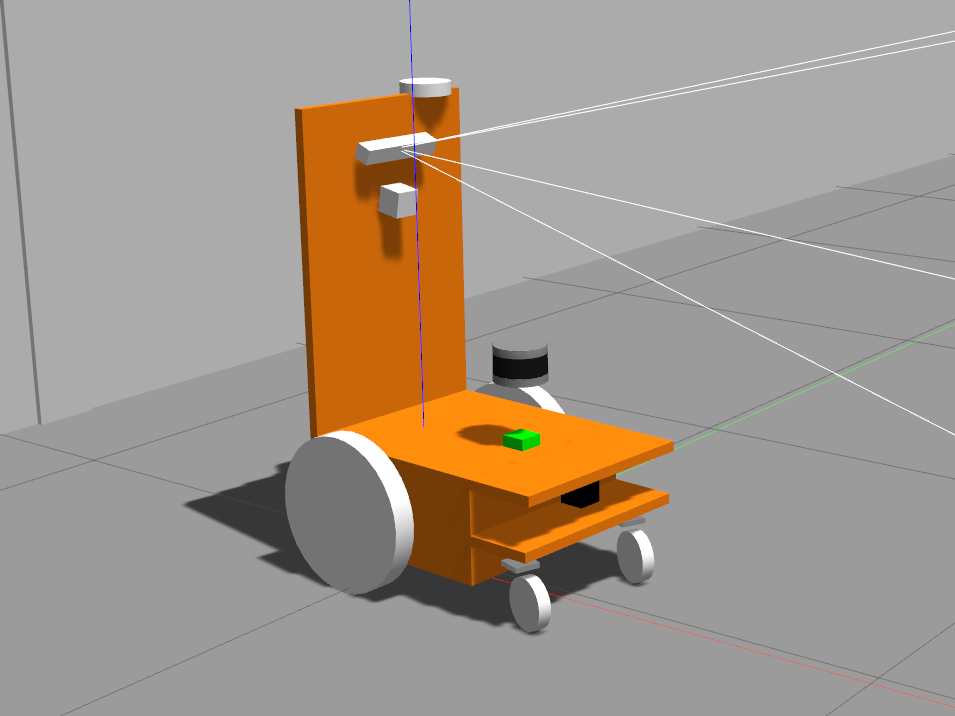
\includegraphics[keepaspectratio, scale=0.15]{images/sim-robot.png}
    \caption{Simulated robot}
    \label{Fig:sim-robot}
  \end{subfigure}
  % \hfill
  \begin{subfigure}{0.40\textwidth}
    \centering
    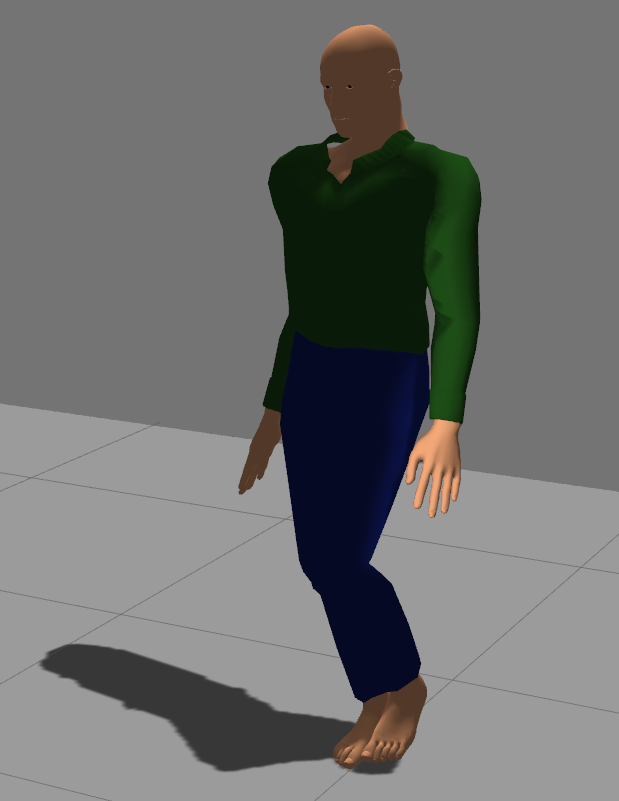
\includegraphics[keepaspectratio, scale=0.15]{images/sim-actor.png}
    \caption{Simulated actor}
    \label{Fig:sim-actor}
  \end{subfigure}
  \caption{Simulated robot and actor}
  \label{Fig:sim-robot-actor}
\end{figure}

% 移動ロボットの自律走行は,つくばチャレンジ2024EX@イーアスつくば\cite{つくばチャレンジ36:online}で千葉工業大学 未来ロボティクス学科 box2チームが完走した際のソフトウェア構成,パラメータを参考にした.これは,Githubで公開されている\cite{openrdco85:online}.なお,後述するシナリオには狭い通路の走行が含まれるため,yaw方向の角速度を小さくなるように変更している.

本研究で用いた移動ロボットの自律走行ソフトウェアおよびパラメータ設定は,つくばチャレンジ2024EX@イーアスつくば\cite{つくばチャレンジ36:online}において,千葉工業大学 未来ロボティクス学科 box2チームが完走した際の構成を参考にしている(Github\cite{openrdco85:online}で公開).なお,後述のシナリオには狭い通路を走行する箇所が含まれているため,yaw方向の角速度を小さくなるように調整している.

\newpage

実験は\figref{Fig:experiment-scenarios}に示す2種類のシナリオで行った.
\figref{Fig:scenario1}のシナリオ1では,ロボットが直線経路を進む途中に歩行者が横断する状況を設定した.\figref{Fig:scenario2}のシナリオ2では,ロボットが狭い通路を走行する際に2名の歩行者がすれ違う状況を設定し,より複雑な環境下でのナビゲーションを想定している.

\begin{figure}[H]
  \centering
  \begin{subfigure}{0.80\textwidth}
    \centering
    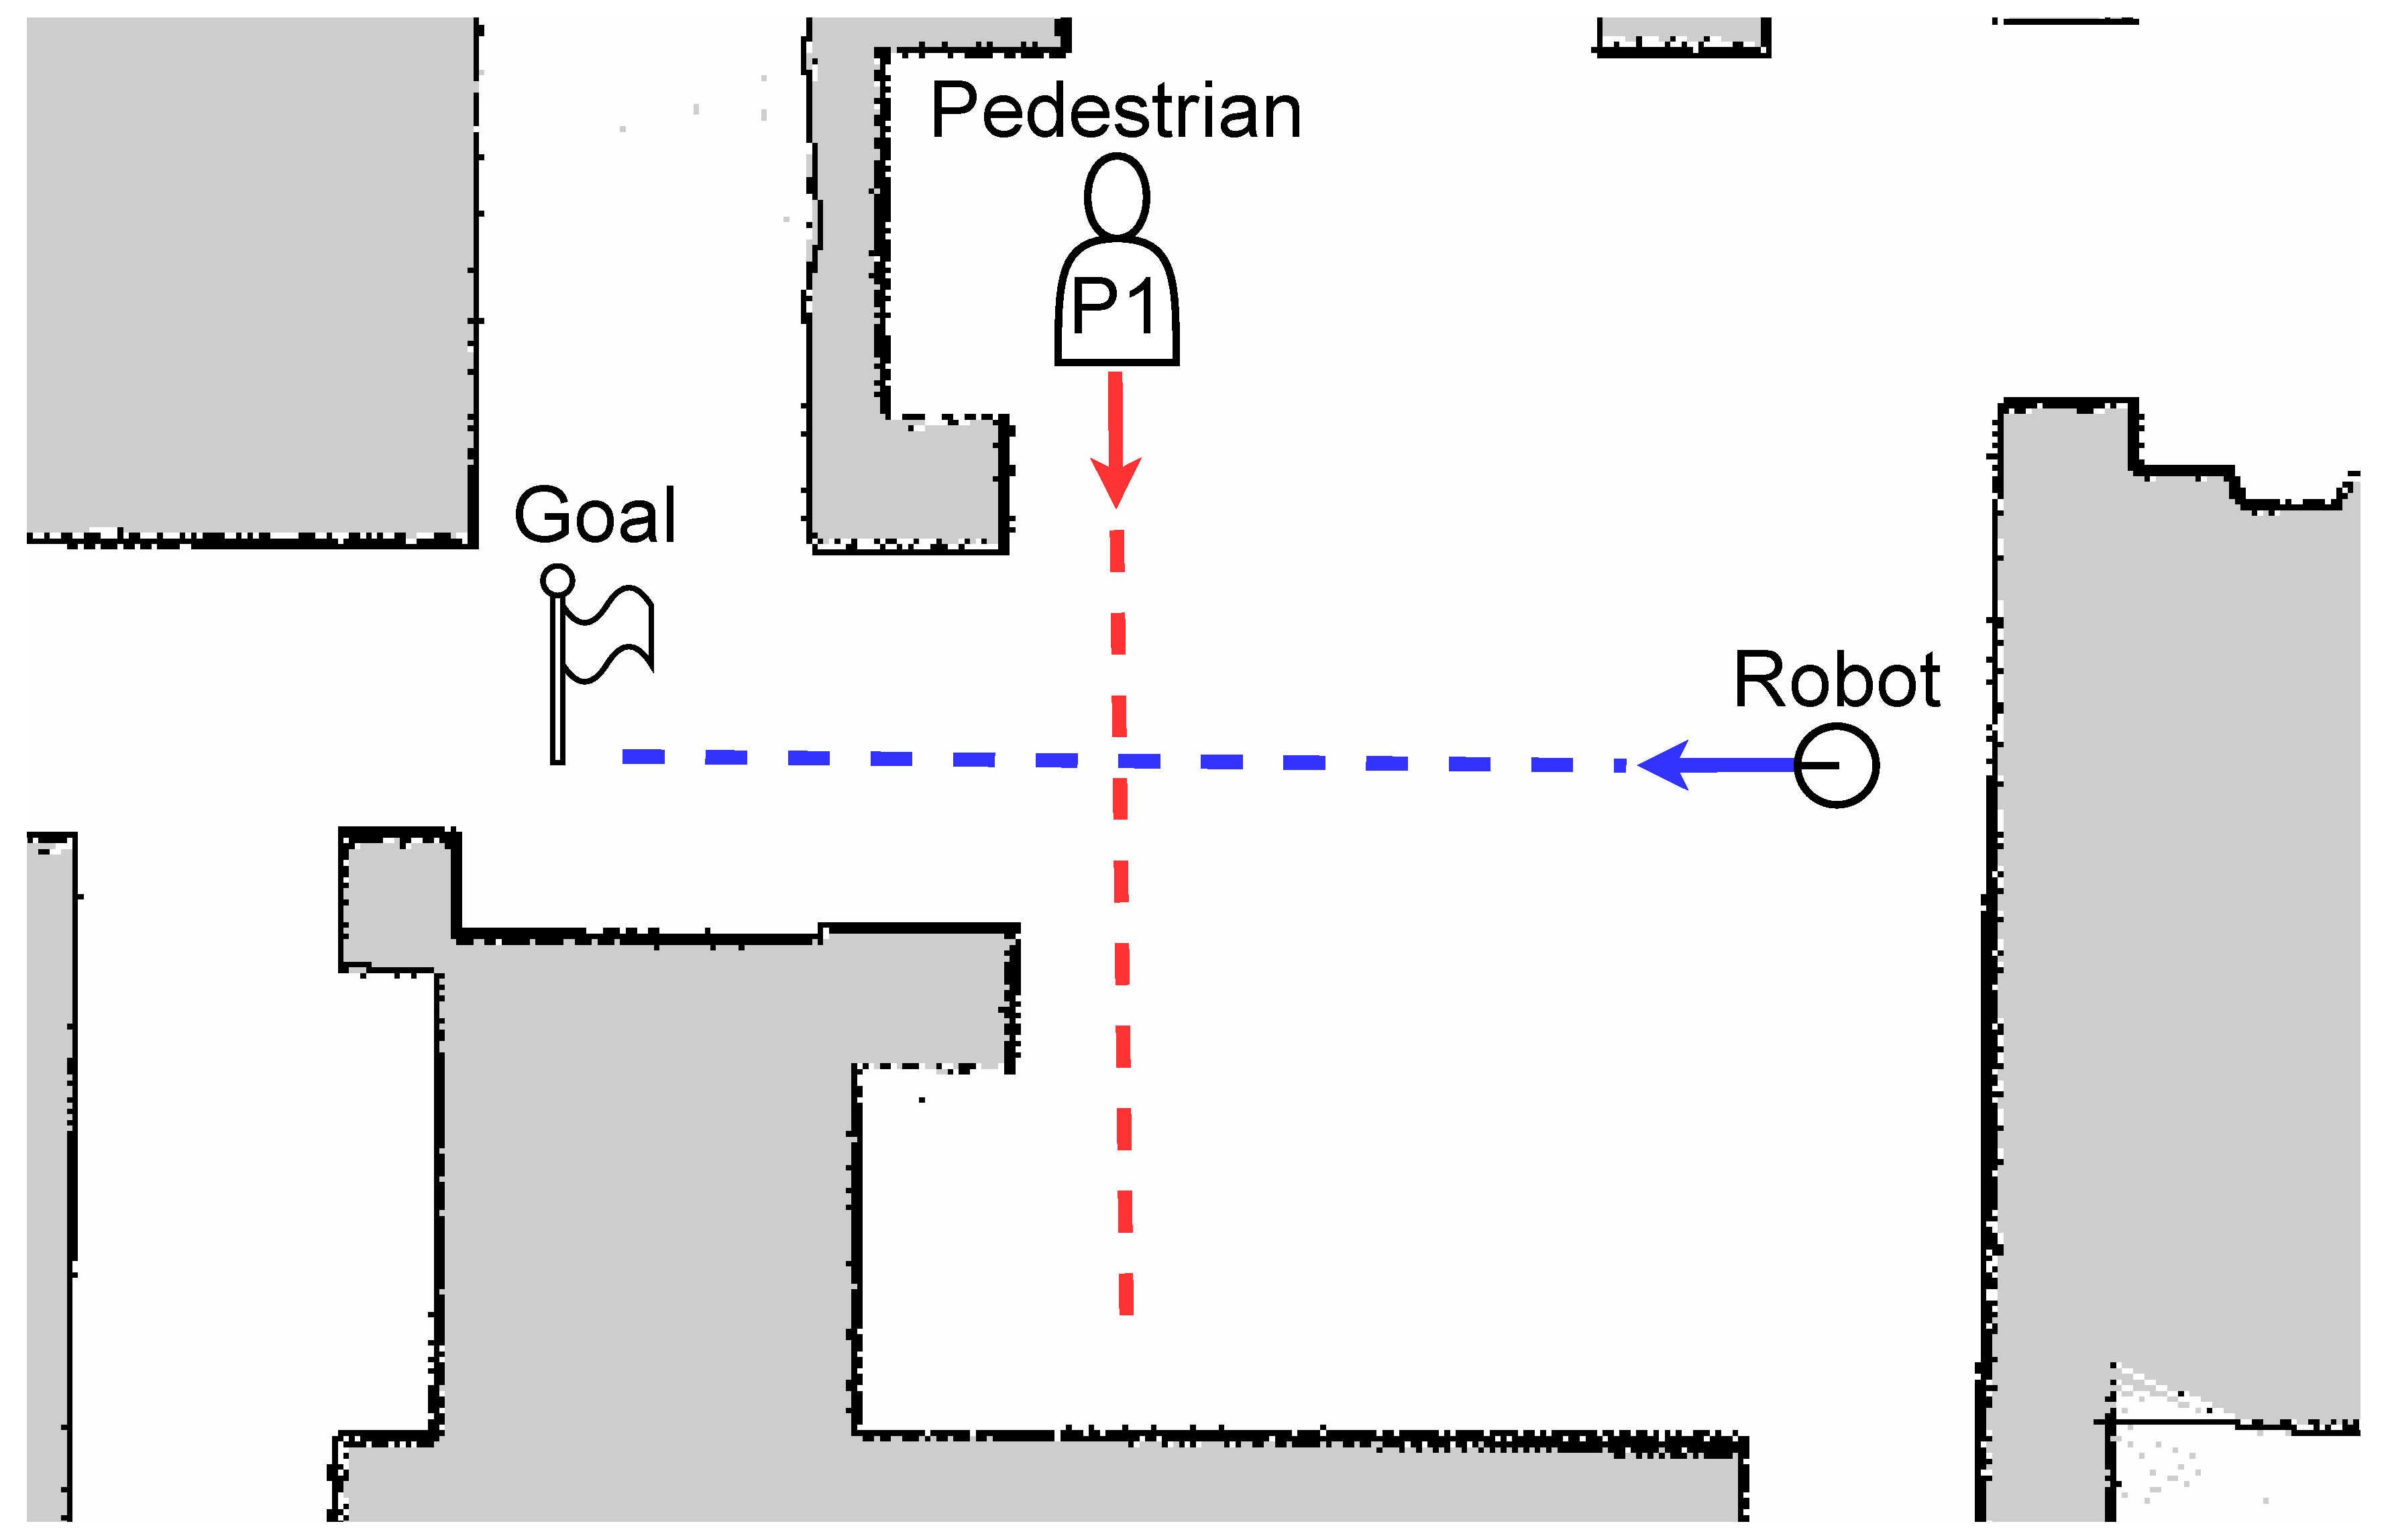
\includegraphics[keepaspectratio, scale=0.15]{images/scenario1.pdf}
    \caption{Scenario 1}
    \label{Fig:scenario1}
  \end{subfigure}
  \vspace{10pt}
  \begin{subfigure}{0.80\textwidth}
    \centering
    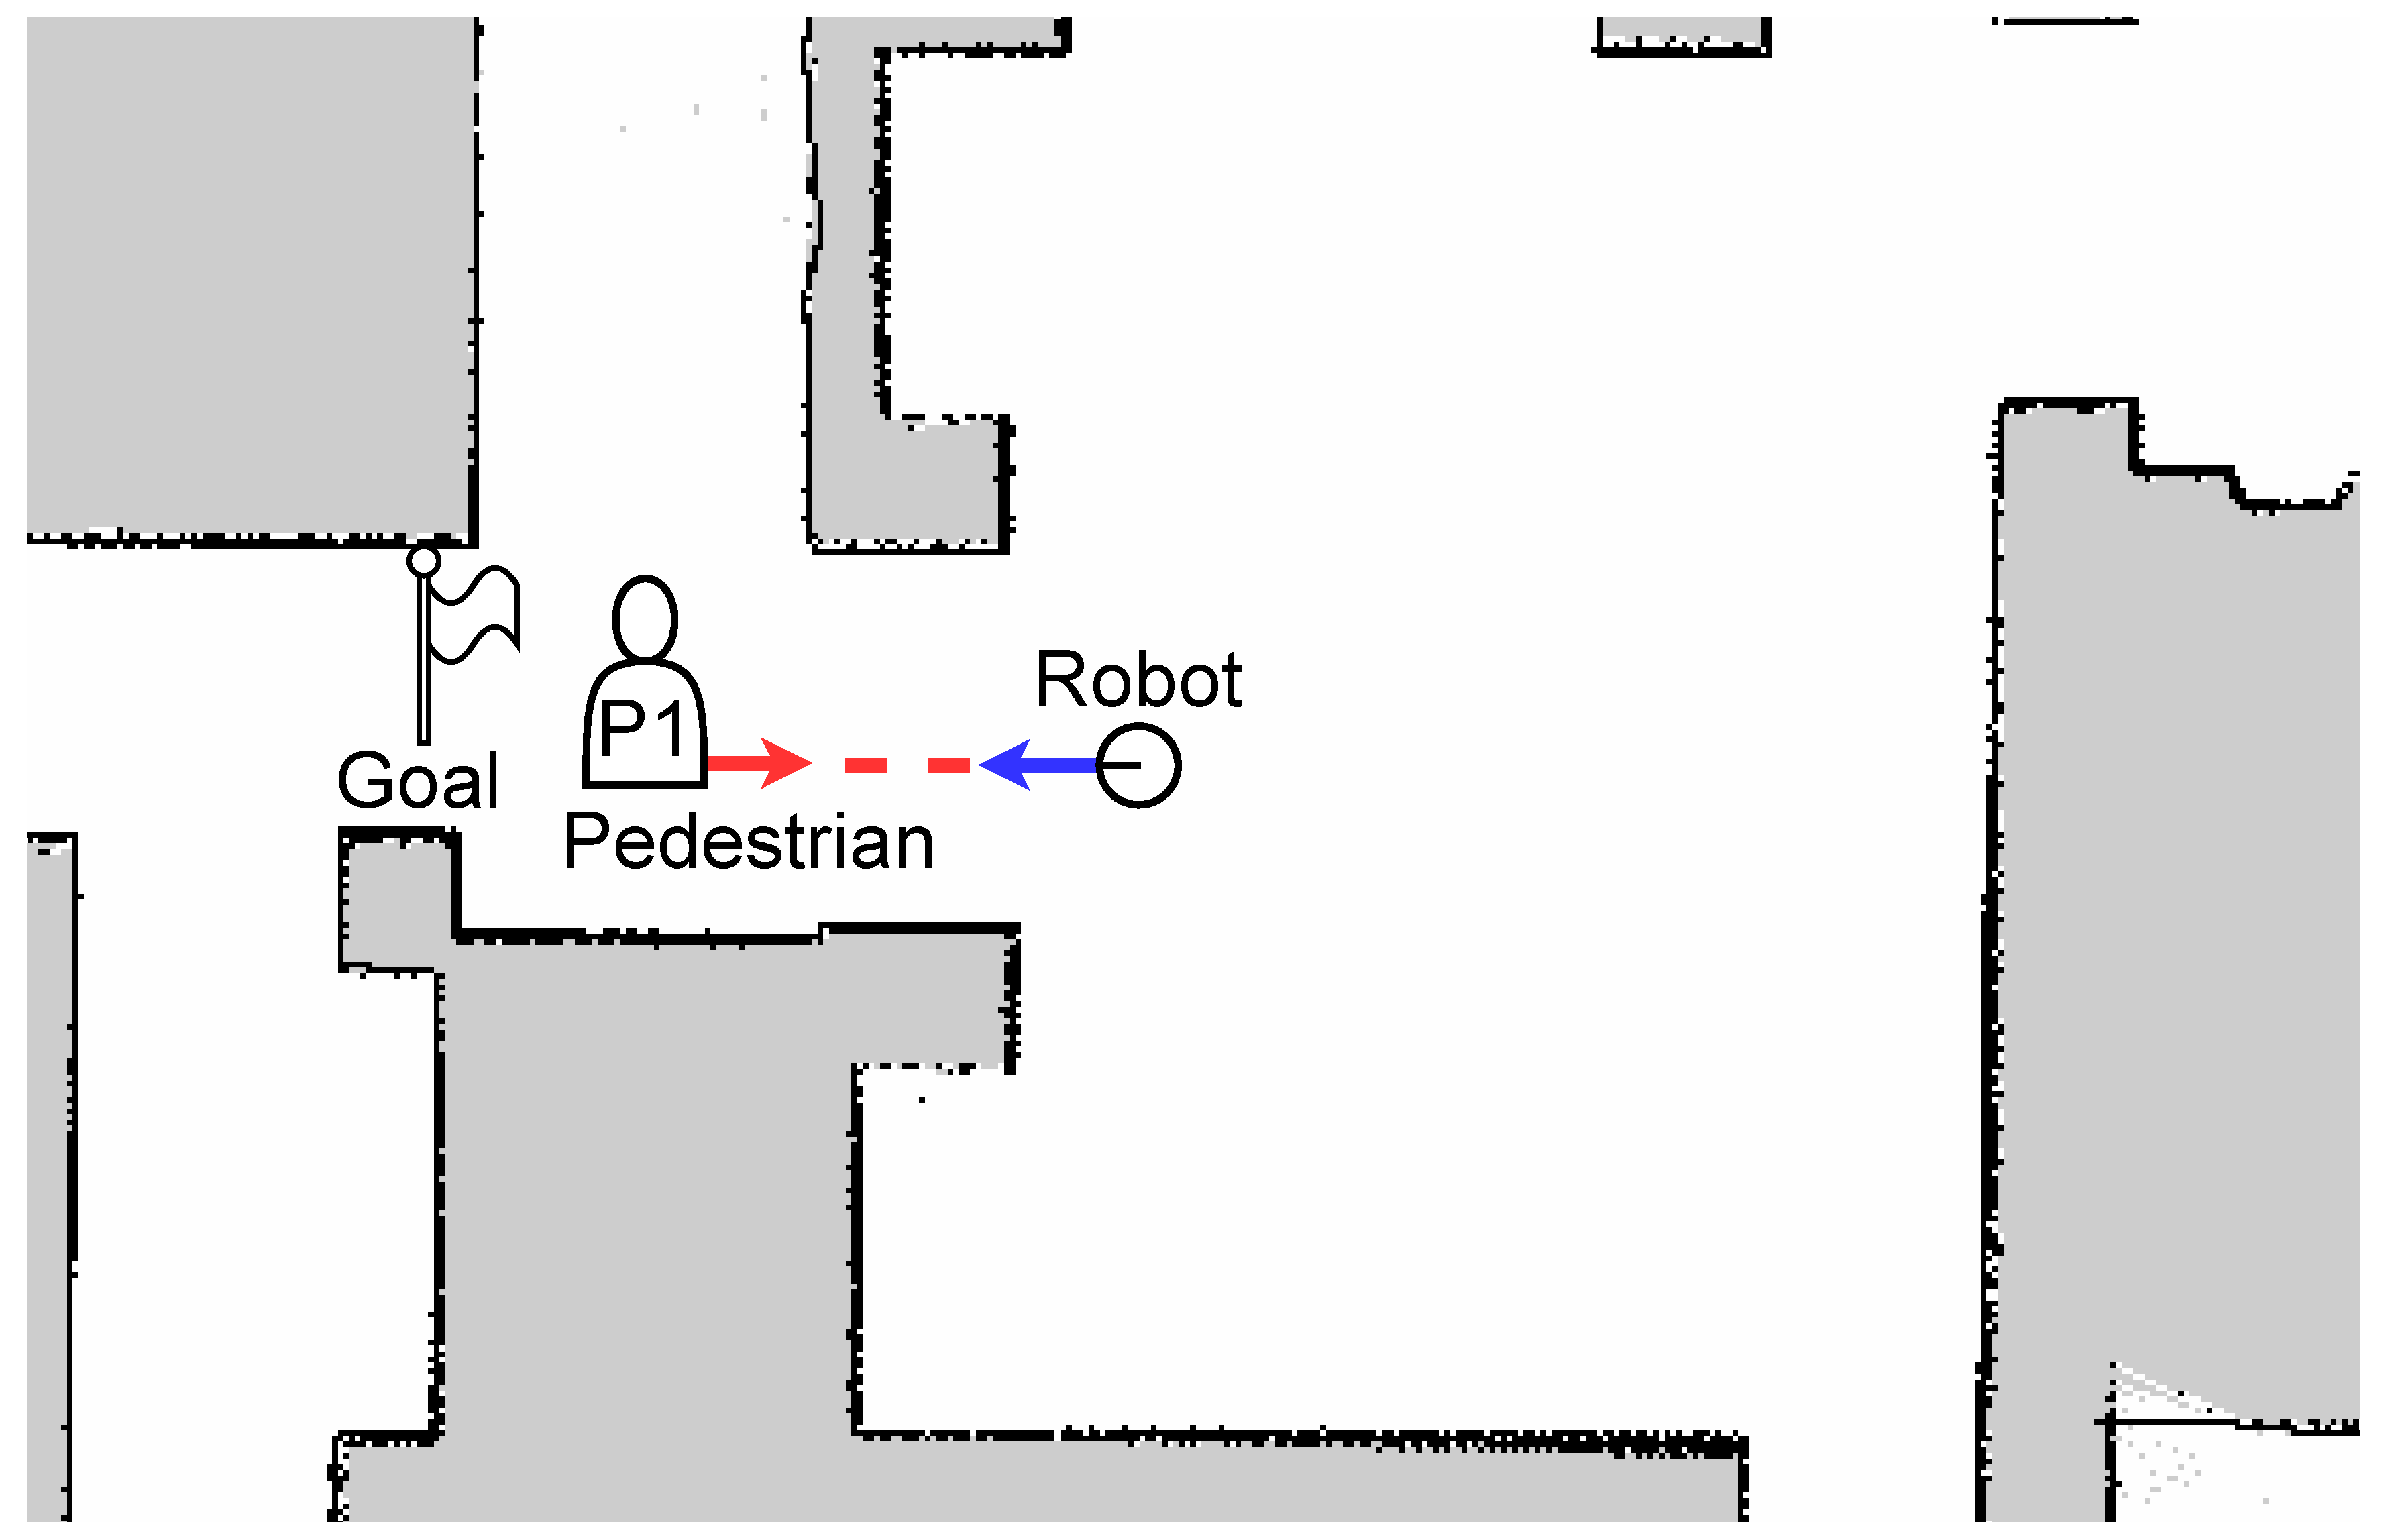
\includegraphics[keepaspectratio, scale=0.15]{images/scenario2.pdf}
    \caption{Scenario 2}
    \label{Fig:scenario2}
  \end{subfigure}
  \caption{Experiment Scenarios}
  \label{Fig:experiment-scenarios}
\end{figure}

\newpage

評価は以下の4項目に基づいて行った.
\begin{itemize}
  \item 走行時間
  \item 走行距離
  \item 歩行者とロボット間の最小距離
  \item 最小のTime to Collision(TTC)
\end{itemize}
ナビゲーションの効率性は走行時間・距離が小さいほど高く,安全性は最小距離・最小TTCが大きいほど高いと考えられる.
TTCは,移動物体同士が現在の速度と進行方向を維持した場合の衝突するまでの時間を示し,以下の式で計算される.
\setlength{\jot}{1em}
\begin{align}
  \mathbf{v}_{robot} = \begin{bmatrix} v_{robot,x} \\ v_{robot,y} \end{bmatrix}, \quad 
  \mathbf{v}_{ped} = \begin{bmatrix} v_{ped,x} \\ v_{ped,y} \end{bmatrix} \\
  \mathbf{v}_{relative} = \mathbf{v}_{robot} - \mathbf{v}_{ped} \\
  \text{TTC} = \frac{\text{d}}{\|\mathbf{v}_{relative}\|}
\end{align}
ここで,$d$はロボットと歩行者の距離,$\mathbf{v}_{robot}$はロボットの速度ベクトル,$\mathbf{v}_{ped}$は歩行者の速度ベクトルである.

\section{結果と考察}\label{sec:exp-sim-result}
\figref{Fig:scenario1-result},\figref{Fig:scenario2-result}は,予測結果を用いないナビゲーションとロボットの行動を考慮した予測結果を用いるナビゲーションの比較結果である.棒グラフは平均値,エラーバーは標準偏差を表す.
まず,\figref{Fig:scenario1-result}に示すシナリオ1の結果を比較すると,走行時間が約1.8倍,走行距離が約1.01倍と悪化した一方で,最小距離が約13倍,最小TTCが約17倍と大幅に改善した.
次に,\figref{Fig:scenario2-result}に示すシナリオ2の結果では,走行時間が約1.5倍,走行距離が約1.01倍,歩行者2の最小距離が0.9倍と悪化したが,歩行者1の最小距離が1.84倍,歩行者1の最小TTCが約1.3倍,歩行者2の最小TTCが約1.1倍と改善した.
これらの結果から,予測結果を用いることで,ロボットのナビゲーションがより安全になる可能性があることが示唆される.一方で,効率性の面では課題が残ることも確認された.

\begin{figure}[H]
  \centering
 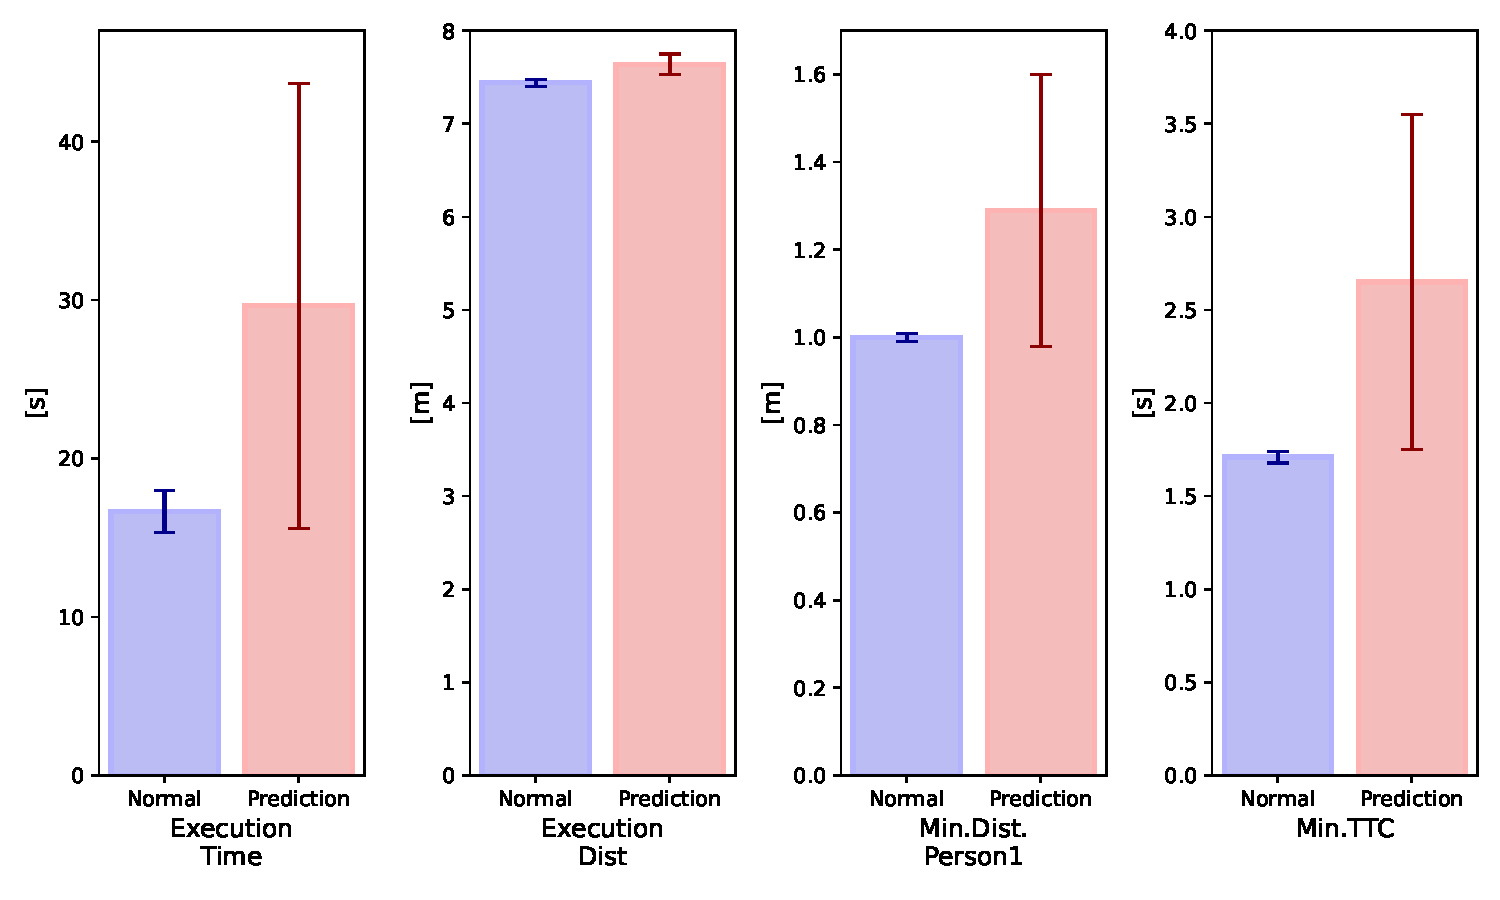
\includegraphics[keepaspectratio, scale=0.53]
      {images/scenario1_result.pdf}
  \caption{Scenario1 result}
 \label{Fig:scenario1-result}
\end{figure} 

\begin{figure}[H]
  \centering
 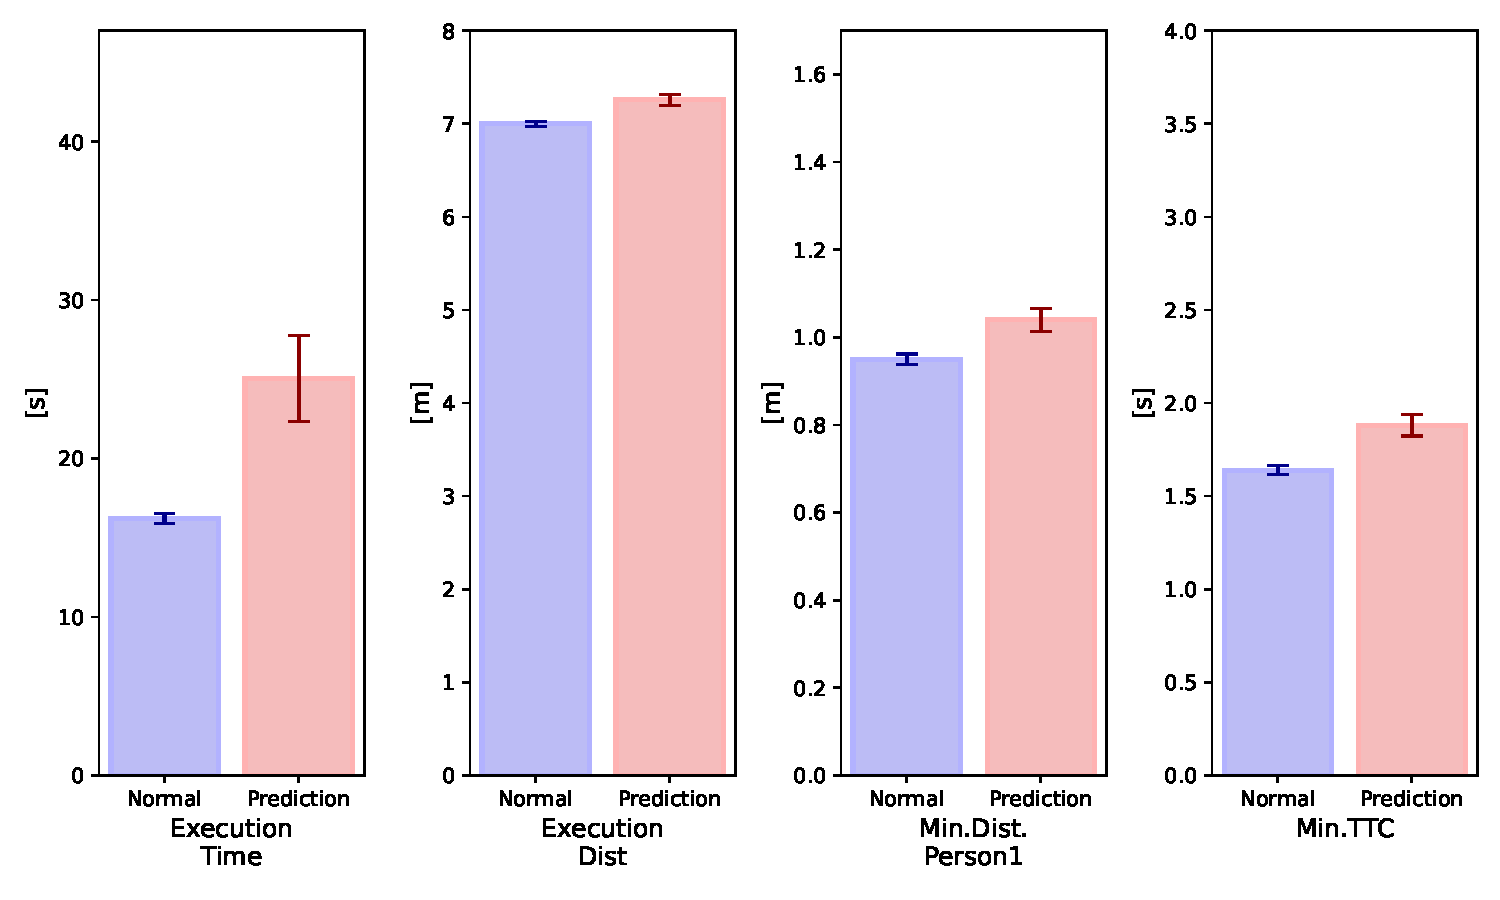
\includegraphics[keepaspectratio, scale=0.44]
      {images/scenario2_result.pdf}
  \caption{Scenario2 result}
 \label{Fig:scenario2-result}
\end{figure} 

\newpage

シナリオ1では,歩行者との最小距離と最小TTCが大幅に改善されており,予測結果を活用することで早期に安全に停止を行い,歩行者との接触リスクを低減できる一方,回避行動に伴う走行時間・距離の増加が生じたと考えられる.つまり,安全性が向上する一方で,効率性の面では課題が残るような結果となった.

シナリオ2では,歩行者1に対する最小距離と最小TTCが改善されているが,歩行者2との最小距離が悪化している.これは,狭い通路でのすれ違い時にロボットが歩行者2に対してより接近する状況が発生したことを意味している.この結果から,狭い空間でのナビゲーションにおいては,予測結果の精度には改善の余地があると考えられる.また,本研究の学習に用いたデータセットはいずれも屋外の広い空間のデータであり,狭い環境での学習サンプルが不足していたことも一因と考えられる.

本実験で用いたシミュレータの歩行者は,一定の線形軌道を常に一定速度で歩行しており,現実の歩行者の動きとは大きく異なっている.つまり,歩行者同士や歩行者とロボット間など,全ての移動体の間に相互作用が存在しない.その結果,相互作用を重視して学習したモデルと実験環境の性質が乖離し,予測性能が低下した可能性がある.さらに,予測結果を用いる場合の標準偏差が大きい要因として,以下の点が考えられる.
\begin{itemize}
  \item 正規分布からサンプリングされた軌道が実際の軌道と大きく異なる場合がある
  \item 0.4秒ごとに反映される予測結果がロボットの経路計画にチャタリングを引き起こす
  \item 前後の予測結果(例えば,$t-1\text{と}t$)に一貫性がない場合がある
\end{itemize}
これらの課題を解決するためには,狭い空間など多様な環境,相互作用を含むデータセットの活用や,提案したナビゲーションシステムの予測結果の扱い方の改善などが今後の検討課題となる.

\newpage
